
\begin{frame}[t,allowframebreaks]{
    Vanishing and exploding gradients -}

    Self-evidently, the method of 
    \index{gradient}\index{gradient descent}\gls{gradient descent}
    requires {\em useful} \index{gradient}\glspl{gradient}.\\
    \vspace{0.2cm}
    Deep neural networks often have 
    training issues associated with either 
    {\bf vanishing} or {\bf exploding} \glspl{gradient}.\\
    \vspace{0.1cm}
    \begin{itemize}
        \small
        \item 
        If the \gls{gradient} is too small, 
        it becomes ineffective or impossible 
        to obtain updates for the network weights,
        especially for the initial layers.
        \item 
        If the \gls{gradient} is too large,
        weight updates become very large destabilising
        the learning process or halting it through numerical overflows. 
    \end{itemize}
    In both cases, {\bf networks becomes unable to learn}.\\
    \vspace{0.2cm}
    Issues arise from the way \glspl{derivative} in
    earlier and later layers are linked.\\
    \begin{itemize}
        \small
        \item
        In \index{back propagation}\gls{back propagation},
        the \glspl{derivative} of the network are found by moving 
        layer by layer, from the final back to the initial one.\\
        \item 
        Using the {\bf chain rule}, \glspl{derivative} of each layer
        are {\bf multiplied across the depth of the network}.
        \item 
        This product of \glspl{derivative} can become
        {\bf problematic for deep networks}, when the product
        includes a large number of terms.
    \end{itemize}

    \framebreak

    %
    %

    Consider a {\bf deep network} with $m$+1 layers, 
    incl. the input/output ones.\\
    Further assume that there is a {\bf single node per layer}.\\
    \vspace{0.2cm}
    Let $x$ (or $y_0$) be the input, $o$ (or $y_m$) the output, and
    $y_{1}, y_{2},...,y_{m-1}$ the output of each of the $m$+1 hidden layers.\\
    \vspace{0.2cm}
    Each computational layer $k$, applies the sigmoid function
    \begin{equation}
        \sigma(z_{k}) = \frac{1}{1+e^{-z_{k}}}
     \end{equation} 
    on its input $z_k$, which is computed as $z_k = w_{k}y_{k-1}+b_{k}$.

    
\begin{center}
    \begin{tikzpicture}[scale=0.8]
   
       %\draw[help lines] (0,0) grid (15,3);
       
       \node[ann_input_node] (x)    
         at ( 1.0, 1.5) {\Large $x$};
       \node[ann_processing_node] (h1)   
         at ( 3.5, 1.5) {\Large $\sigma$};
       \node[ann_processing_node] (h2)   
         at ( 6.0, 1.5) {\Large $\sigma$};
       \node[ann_processing_node_rep] (hi)   
         at ( 8.5, 1.5) {\Large $...$};
       \node[ann_processing_node] (hm_1) 
         at (11.5, 1.5) {\Large $\sigma$};
       \node[ann_processing_node] (o)    
         at (14.5, 1.5) {\Large $\sigma$};       

       \drawgraphlinebigarrow (x.east)       
         to[left =0] 
           node[above,midway,xshift=0.4cm,yshift=0.3cm]
             {$z_1$}
           node[below,midway,xshift=0.0cm,yshift=-0.2cm]
             {$w_1,b_1$}
         (h1.west) ;

       \drawgraphlinebigarrow (h1.east)       
         to[left =0] 
           node[above,midway,xshift=-0.4cm,yshift=0.3cm]
             {$y_1$}
           node[above,midway,xshift=0.4cm,yshift=0.3cm]
             {$z_2$}
           node[below,midway,xshift=0.0cm,yshift=-0.2cm]
             {$w_2,b_2$}
         (h2.west) ;

       \drawgraphlinebigarrow (h2.east)       
         to[left =0] 
           node[above,midway,xshift=-0.4cm,yshift=0.3cm]
             {$y_2$}
           node[below,midway,xshift=0.0cm,yshift=-0.2cm]
             {$w_3,b_3$}
         (hi.west) ;

       \drawgraphlinebigarrow (hi.east)       
         to[left =0] 
           node[above,midway,xshift=0.3cm,yshift=0.3cm]
             {$z_{m-1}$}
           node[below,midway,xshift=-0.1cm,yshift=-0.2cm]
             {$w_{m-1},b_{m-1}$}
         (hm_1.west) ;

       \drawgraphlinebigarrow (hm_1.east)       
         to[left =0] 
           node[above,midway,xshift=-0.4cm,yshift=0.3cm]
             {$y_{m-1}$}
           node[above,midway,xshift=0.5cm,yshift=0.3cm]
             {$z_{m}$}
           node[below,midway,xshift=0.0cm,yshift=-0.2cm]
             {$w_{m},b_{m}$}
         (o.west) ;

       \drawgraphlinebigarrow (o.east)       
         to[left =0] 
           node[above,midway,xshift=-0.1cm,yshift=0.3cm]
             {$o$}
         (15.8,1.5) ;
         
    \end{tikzpicture}
\end{center}


    \framebreak

    %
    %

    \vspace{-1.0cm}

    Therefore, the network evaluates the following expressions:
    \begin{equation}
       o = \sigma(z_m) = \sigma(w_{m} y_{m-1} + b_{m}) 
    \end{equation}
    \begin{equation}
        y_{m-1} = \sigma(z_{m-1}) = \sigma(w_{m-1} y_{m-2} + b_{m-1}) 
     \end{equation}
     \begin{equation*}
        \cdots
     \end{equation*}
     \begin{equation}
        y_{2} = \sigma(z_{2}) = \sigma(w_{2} y_{1} + b_{2}) 
     \end{equation}
     \begin{equation}
        y_{1} = \sigma(z_{1}) = \sigma(w_{1} x + b_{1}) 
     \end{equation}
     building up the following composite function:
     \begin{equation}
        o = \sigma\Bigg( 
               w_{m} \bigg( 
                  \sigma\Big(
                     w_{m-1} \sigma\big(
                     \cdots
                     w_{2}\sigma(w_{1} x + b_{1})+b_{2}
                     \cdots \big) + b_{m-1}
                  \Big) 
               \bigg) + b_{m} 
            \Bigg) 
     \end{equation}
  
    \framebreak

    %
    %

    Let $\displaystyle \partial L/\partial w_{1}$
    be the derivative of the loss function, $L$, 
    with respect to the weight of the initial layer $w_1$.
    The chain rule yields:
    \begin{equation}
        \frac{\partial L}{\partial w_{1}} = 
            \frac{\partial L}{\partial o}  \cdot
            \frac{\partial o}{\partial y_{m-1}}  \cdot
            \frac{\partial y_{m-1}}{\partial y_{m-2}} \cdot  
            \cdots
            \frac{\partial y_{2}}{\partial y_{1}} \cdot 
            \frac{\partial y_{1}}{\partial w_{1}}  
            \label{eq:dL_dw1_backpropagation_1}
    \end{equation}
    where:
    \begin{equation}
            \frac{\partial y_{1}}{\partial w_{1}}  =
              \sigma^{\prime}(z_{1}) x
    \end{equation}

    \begin{equation}
        \frac{\partial y_{2}}{\partial y_{1}}  =
          \sigma^{\prime}(z_{2}) w_{2}
    \end{equation}

    \begin{equation*}
        \cdots
    \end{equation*}

    \begin{equation}
        \frac{\partial o}{\partial y_{m-1}}  =
          \sigma^{\prime}(z_{m}) w_{m}
    \end{equation}

    \framebreak

    %
    %

    The evaluation of 
    $\displaystyle \partial L/\partial w_{1}$,
    using Eq.~\ref{eq:dL_dw1_backpropagation_1}, 
    requires the calculation of the product:
    \begin{equation*}
        \sigma^{\prime}(z_{1}) 
        \sigma^{\prime}(z_{2}) 
        \cdots
        \sigma^{\prime}(z_{m})
    \end{equation*}    

    \begin{columns}
        \begin{column}{0.50\textwidth}        
            \begin{center}
                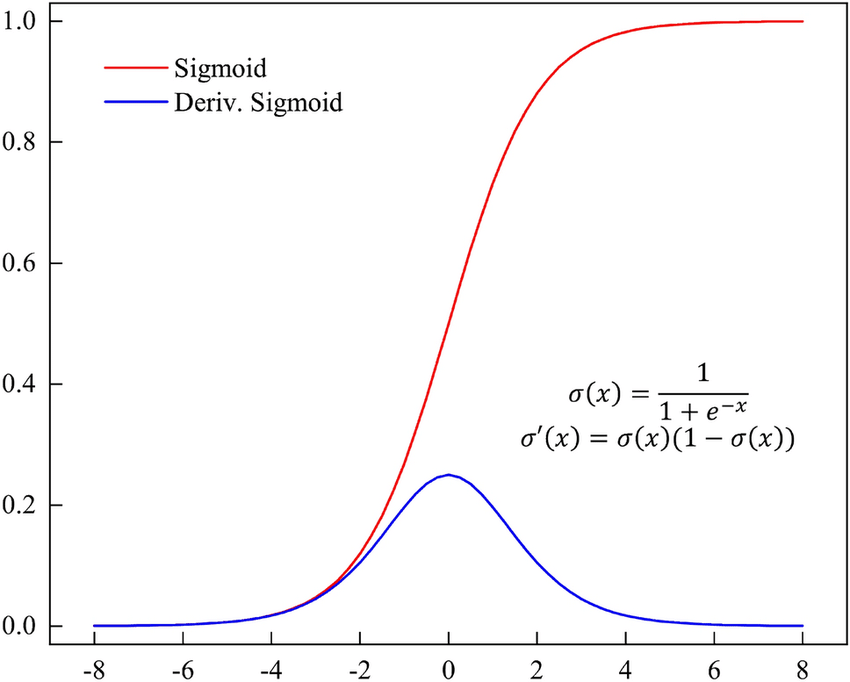
\includegraphics[width=1.00\textwidth]
                    {./images/activation_functions/xiang22_sigmoid_and_derivative.png}\\
                {\tiny 
                    \color{col:attribution} 
                    Schematic taken from Fig. 6 in \cite{Xiang:2022ato}.\\
                }
            \end{center}        
        \end{column}
        \begin{column}{0.50\textwidth}
            The \index{sigmoid}\gls{sigmoid} 
            \index{activation function}\gls{activation function},
            has a \gls{derivative} that is
            is always $<$ 1.\\
            \begin{itemize}
                \small
                \item It is only 0.25 at its maximum.\\
            \end{itemize}
            \vspace{0.2cm}
            After $N$ layers, the gradient contains
            a factor $<0.25^N$.        
            \begin{itemize}
                \small
                \item With 20 layers, $0.25^{20} \approx 10^{-12}$.
            \end{itemize}
            \vspace{0.2cm}
            Therefore, using 
            \index{back propagation}\gls{back propagation},
            the early network layers receive vanishingly small
            weight updates.
        \end{column}
    \end{columns}

    \framebreak

    %
    %

    Possible solutions to the 
    \index{vanishing gradient}\gls{vanishing gradient} 
    problem include:

    \begin{itemize}
        \item {\bf Using a different activation function} 
        \begin{itemize}
            \small
            \item 
            For example, the \index{ReLU}\gls{relu} (see figure below)
        \end{itemize}
        \item {\bf Initializing the network with large weights}
        \begin{itemize}
            \small
            \item 
            This is motivated by the fact that the product of weights also enters in the
            calculation of the \glspl{derivative} of the 
            \gls{loss function}
            (see Eq.~\ref{eq:dL_dw1_backpropagation_1}).
        \end{itemize}
    \end{itemize}

    \begin{center}
        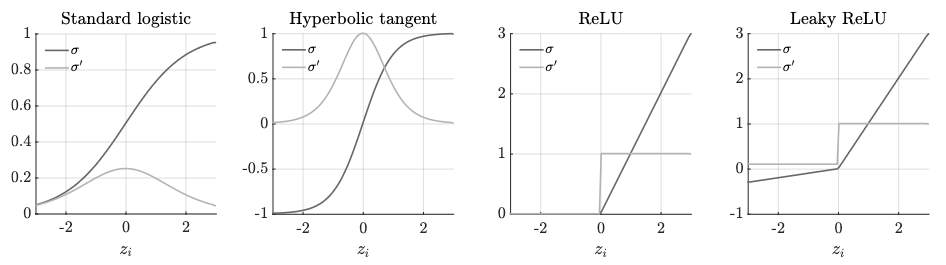
\includegraphics[width=0.99\textwidth]
            {./images/activation_functions/ostwald21_common_activation_functions_and_derivatives.png}\\
        {\tiny 
            Common activation functions and their derivatives.
            \color{col:attribution} 
            Taken from Fig. 1 in \cite{Ostwald:2021bpi}.\\
        }
    \end{center}        

    \framebreak

    %
    %

    However, these ``solutions'' to the
    \index{vanishing gradient}\gls{vanishing gradient} problem
    can cause the \gls{gradient} 
    to increase exponentially 
    along the depth of the network.
    \begin{itemize}
    \item This exponential increase is known as the 
     \index{exploding gradient}\gls{exploding gradient} problem.\\
    \end{itemize}

    Different strategies are then used to mitigate the 
    \gls{exploding gradient} problem:
    \begin{itemize}
        \item 
         \gls{gradient} clipping.\\
    \end{itemize}    
    \vspace{0.3cm}

    The
    \index{vanishing gradient}\gls{vanishing gradient} and
    \index{exploding gradient}\gls{exploding gradient} problems are
    {\bf inherent to multivariable optimization}$^1$.\\

    \vspace{0.4cm}

    \noindent\rule{4cm}{0.4pt}\\
    {
    \scriptsize
    $^1$ Although the previous observations were made for a simple network
    with a single node per layer, they are also valid for more complex networks.\\
    \begin{itemize}
        \scriptsize
        \item In the more general case, a layer-to-layer 
        \index{back propagation}\gls{back propagation} update includes 
        a (\index{Jacobian}\gls{Jacobian}) matrix (rather than scalar) multiplication         
        \cite{Aggarwal:2018SpringerDL}.
        \item Repeated matrix multiplications as unstable as
        repeated scalar ones.
    \end{itemize}
    }

    \framebreak

    %
    %

    Consider the following examples of two simple, bivariate 
    \index{loss function}\glspl{loss function}, $L$:\\
    \vspace{-0.2cm}
    \begin{equation}
        L(x,y) = 
        \begin{cases}
            x^2 + y^2,  & \text{example A} \\
            x^2 + 4y^2, & \text{example B}
        \end{cases}
    \end{equation}

    \vspace{-0.3cm}

    In example A:\\
    \begin{itemize}
        \small
        \item The \gls{loss function} looks like a {\bf circular} bowl
        (a {\em special} case) and treats the variables $x$ and $y$ symmetrically.
        \item The negative \gls{gradient} of $L$ at any point in the 
        $(x,y)$ space points directly to the minimum of $L$.\\
    \end{itemize}

    In example B:\\
    \begin{itemize}
        \small
        \item The \gls{loss function} looks like an {\bf elliptical} bowl
        and, for a unit change in the input variables,
        $y$ contributes significantly more to the loss.
        \begin{itemize}
            \small
            \item We say that $L$ is {\em more sensitive} to $y$.
        \end{itemize}    
        \item The negative \gls{gradient} of $L$ at $(x,y)$ is only
        an {\bf instantaneous direction} of best movement and does not point
        towards the minimum of $L$.
        \begin{itemize}
            \small
            \item The \gls{gradient} is {\em weighted 
            more heavily} in the $y$ direction.
        \end{itemize}    
    \end{itemize}

    \framebreak

    %
    %

    With very few exceptions, the {\bf instantaneous direction} 
    of best movement is {\bf not the correct direction of 
    descent in the longer term}.\\

    \vspace{0.2cm}

    \begin{center}
        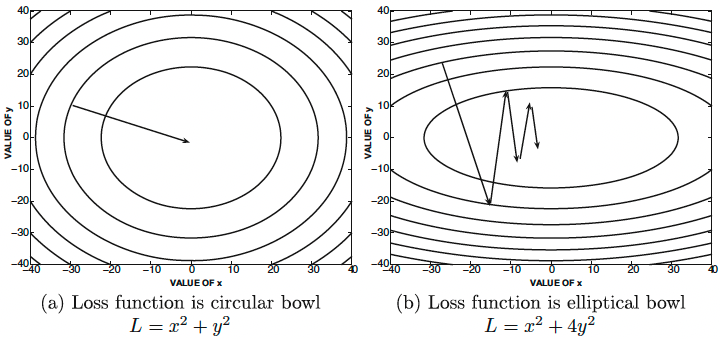
\includegraphics[width=0.99\textwidth]
            {./images/training_issues/aggarwal18_shape_loss_function_grad_descent.png}\\
        {\tiny 
            \color{col:attribution} 
            Fig. 3.9 in \cite{Aggarwal:2018SpringerDL}.\\
        }
    \end{center}        

    \framebreak

    %
    %

    If the instantaneous direction of best movement 
    not the correct direction of 
    descent in the longer term, then one needs to:
    \begin{itemize}
        \item take only a small step, and
        \item calculate a course correction.
    \end{itemize}    

    \vspace{0.2cm}

    With \index{vanishing gradient}\glspl{vanishing gradient},
    our \index{optimisation}\gls{optimisation} procedure 
    is forced to make an {\bf extremely large number of iterations},
    which is {\bf inefficient}.

\end{frame}
